\documentclass{standalone}
\usepackage{xcolor}
\usepackage{tikz}
\usetikzlibrary{positioning, shapes.multipart, calc, graphs, graphs.standard, arrows.meta}
\begin{document}
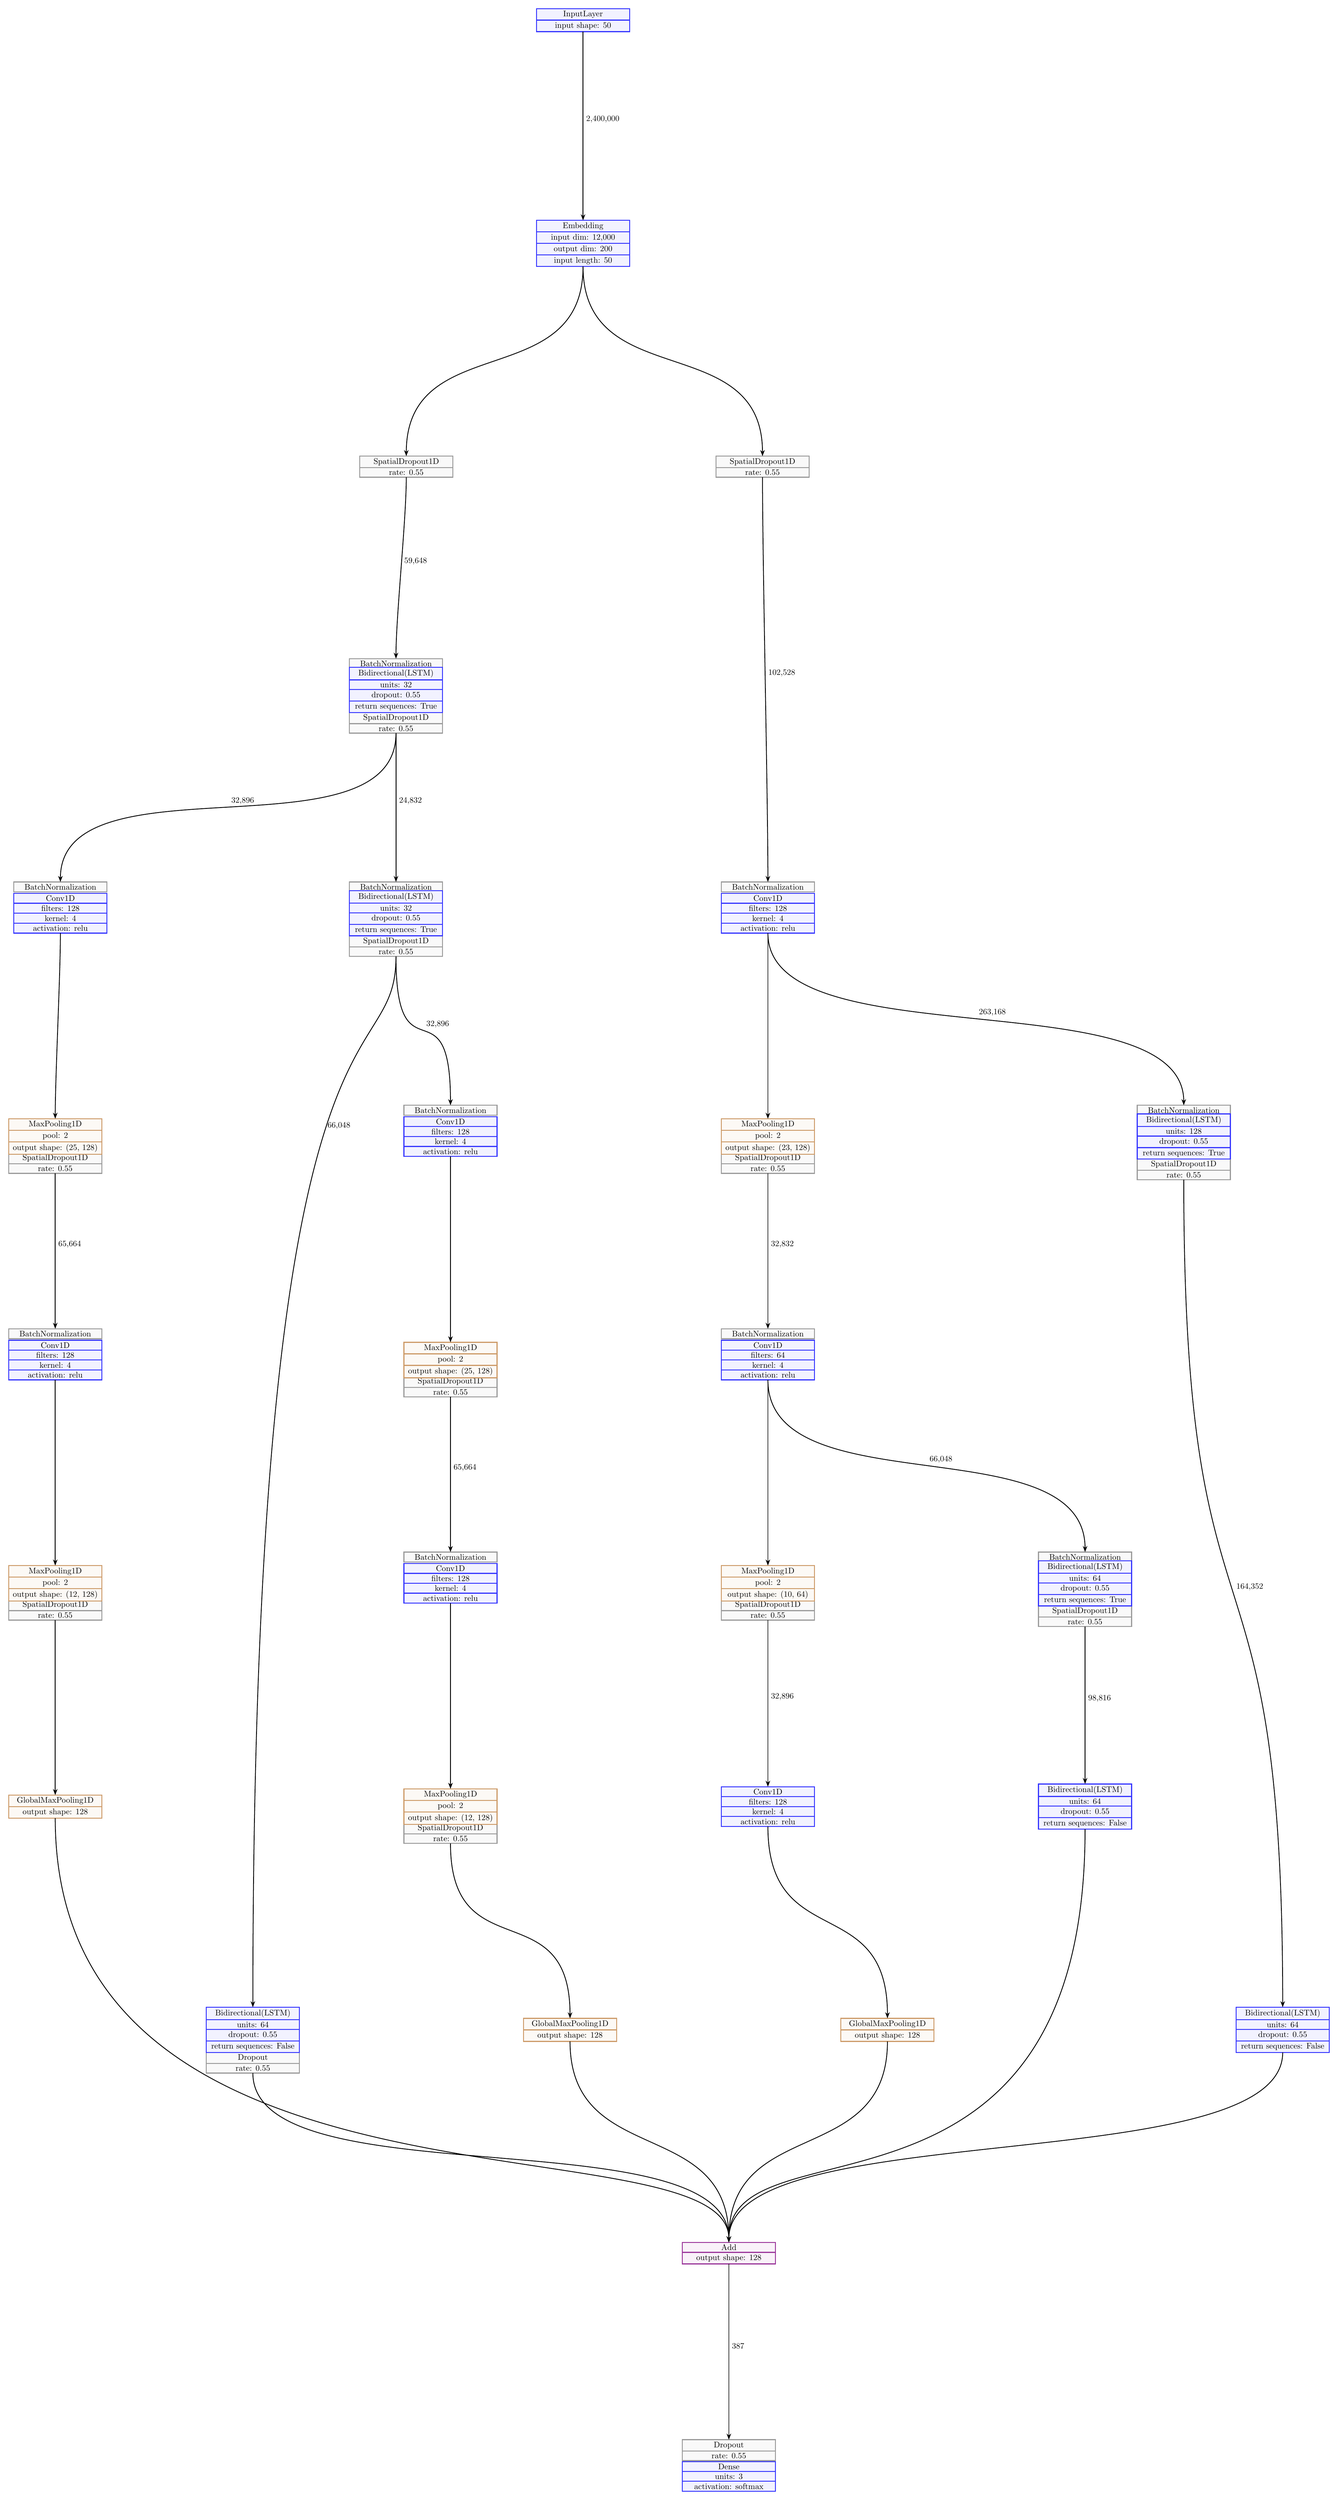
\begin{tikzpicture}[x=15.0pt, y=15.0pt, scale=2.0]
% style: major_grid
\tikzstyle{major_grid}=[black,step=20pt]
% style: minor_grid
\tikzstyle{minor_grid}=[very thin,step=10pt]
% style: defaultEdge
\tikzstyle{defaultEdge}=[thick,out=-90,in=90,out distance=1.5cm,in distance=1.5cm,looseness=1.5]
% style: defaultLabel
\tikzstyle{defaultLabel}=[auto,anchor=south west]
% style: operation_layer_style
\tikzstyle{operation_layer_style}=[rectangle split,rectangle split ignore empty parts,very thick,rectangle split parts=5,draw=violet!80,fill=violet!5,minimum width=4cm,outer sep=0cm,inner sep=2pt]
% style: pool_layer_style
\tikzstyle{pool_layer_style}=[rectangle split,rectangle split ignore empty parts,very thick,rectangle split parts=5,draw=brown!80,fill=brown!5,minimum width=4cm,outer sep=0cm,inner sep=2pt]
% style: utility_layer_style
\tikzstyle{utility_layer_style}=[rectangle split,rectangle split ignore empty parts,very thick,rectangle split parts=5,draw=gray!80,fill=gray!5,minimum width=4cm,outer sep=0cm,inner sep=2pt]
% style: default_layer_style
\tikzstyle{default_layer_style}=[rectangle split,rectangle split ignore empty parts,very thick,rectangle split parts=5,draw=blue!80,fill=blue!5,minimum width=4cm,outer sep=0cm,inner sep=2pt]
% style: misc_layer_style
\tikzstyle{misc_layer_style}=[rectangle split,rectangle split ignore empty parts,very thick,rectangle split parts=5,draw=teal!80,fill=teal!5,minimum width=4cm,outer sep=0cm,inner sep=2pt]

\definecolor{COLOR0}{RGB}{253,231,199}
\definecolor{COLOR1}{RGB}{253,211,157}
\definecolor{COLOR2}{RGB}{252,186,131}
\definecolor{COLOR3}{RGB}{251,140,88}
\definecolor{COLOR4}{RGB}{238,99,71}
\definecolor{COLOR5}{RGB}{214,46,30}
\definecolor{COLOR6}{RGB}{177,0,0}
% node group: input_5_group
% node: input_5
\node[default_layer_style] (input_5) at (21.5, 100.0)
    {
    \nodepart{one}{InputLayer}
    \nodepart{two}{input shape: 50}};
% end of node group: input_5_group

% node group: embedding_1_group
% node: embedding_1
\node[default_layer_style] (embedding_1) at (21.5, 90.91)
    {
    \nodepart{one}{Embedding}
    \nodepart{two}{input dim: 12,000}
    \nodepart{three}{output dim: 200}
    \nodepart{four}{input length: 50}};
% end of node group: embedding_1_group

% node group: spatial_dropout1d_12_group
% node: spatial_dropout1d_12
\node[utility_layer_style] (spatial_dropout1d_12) at (14.3, 81.82)
    {
    \nodepart{one}{SpatialDropout1D}
    \nodepart{two}{rate: 0.55}};
% end of node group: spatial_dropout1d_12_group

% node group: spatial_dropout1d_19_group
% node: spatial_dropout1d_19
\node[utility_layer_style] (spatial_dropout1d_19) at (28.81, 81.82)
    {
    \nodepart{one}{SpatialDropout1D}
    \nodepart{two}{rate: 0.55}};
% end of node group: spatial_dropout1d_19_group

% node group: bidirectional_7_group
% node: batch_normalization_32
\node[utility_layer_style] (batch_normalization_32) at (13.88, 73.8)
    {
    \nodepart{one}{BatchNormalization}};
% node: spatial_dropout1d_13
\node[utility_layer_style] (spatial_dropout1d_13) at (13.88, 71.4)
    {
    \nodepart{one}{SpatialDropout1D}
    \nodepart{two}{rate: 0.55}};
% node: bidirectional_7
\node[default_layer_style] (bidirectional_7) at (13.88, 72.73)
    {
    \nodepart{one}{Bidirectional(LSTM)}
    \nodepart{two}{units: 32}
    \nodepart{three}{dropout: 0.55}
    \nodepart{four}{return sequences: True}};
% end of node group: bidirectional_7_group

% node group: conv1d_11_group
% node: batch_normalization_38
\node[utility_layer_style] (batch_normalization_38) at (29.03, 64.71)
    {
    \nodepart{one}{BatchNormalization}};
% node: conv1d_11
\node[default_layer_style] (conv1d_11) at (29.03, 63.64)
    {
    \nodepart{one}{Conv1D}
    \nodepart{two}{filters: 128}
    \nodepart{three}{kernel: 4}
    \nodepart{four}{activation: relu}};
% end of node group: conv1d_11_group

% node group: max_pooling1d_10_group
% node: spatial_dropout1d_21
\node[utility_layer_style] (spatial_dropout1d_21) at (29.03, 53.48)
    {
    \nodepart{one}{SpatialDropout1D}
    \nodepart{two}{rate: 0.55}};
% node: max_pooling1d_10
\node[pool_layer_style] (max_pooling1d_10) at (29.03, 54.55)
    {
    \nodepart{one}{MaxPooling1D}
    \nodepart{two}{pool: 2}
    \nodepart{three}{output shape: (23, 128)}};
% end of node group: max_pooling1d_10_group

% node group: bidirectional_10_group
% node: batch_normalization_39
\node[utility_layer_style] (batch_normalization_39) at (45.97, 55.62)
    {
    \nodepart{one}{BatchNormalization}};
% node: spatial_dropout1d_20
\node[utility_layer_style] (spatial_dropout1d_20) at (45.97, 53.22)
    {
    \nodepart{one}{SpatialDropout1D}
    \nodepart{two}{rate: 0.55}};
% node: bidirectional_10
\node[default_layer_style] (bidirectional_10) at (45.97, 54.55)
    {
    \nodepart{one}{Bidirectional(LSTM)}
    \nodepart{two}{units: 128}
    \nodepart{three}{dropout: 0.55}
    \nodepart{four}{return sequences: True}};
% end of node group: bidirectional_10_group

% node group: conv1d_7_group
% node: batch_normalization_33
\node[utility_layer_style] (batch_normalization_33) at (0.21, 64.71)
    {
    \nodepart{one}{BatchNormalization}};
% node: conv1d_7
\node[default_layer_style] (conv1d_7) at (0.21, 63.64)
    {
    \nodepart{one}{Conv1D}
    \nodepart{two}{filters: 128}
    \nodepart{three}{kernel: 4}
    \nodepart{four}{activation: relu}};
% end of node group: conv1d_7_group

% node group: bidirectional_8_group
% node: batch_normalization_35
\node[utility_layer_style] (batch_normalization_35) at (13.88, 64.71)
    {
    \nodepart{one}{BatchNormalization}};
% node: spatial_dropout1d_16
\node[utility_layer_style] (spatial_dropout1d_16) at (13.88, 62.31)
    {
    \nodepart{one}{SpatialDropout1D}
    \nodepart{two}{rate: 0.55}};
% node: bidirectional_8
\node[default_layer_style] (bidirectional_8) at (13.88, 63.64)
    {
    \nodepart{one}{Bidirectional(LSTM)}
    \nodepart{two}{units: 32}
    \nodepart{three}{dropout: 0.55}
    \nodepart{four}{return sequences: True}};
% end of node group: bidirectional_8_group

% node group: max_pooling1d_6_group
% node: spatial_dropout1d_14
\node[utility_layer_style] (spatial_dropout1d_14) at (0.0, 53.48)
    {
    \nodepart{one}{SpatialDropout1D}
    \nodepart{two}{rate: 0.55}};
% node: max_pooling1d_6
\node[pool_layer_style] (max_pooling1d_6) at (0.0, 54.55)
    {
    \nodepart{one}{MaxPooling1D}
    \nodepart{two}{pool: 2}
    \nodepart{three}{output shape: (25, 128)}};
% end of node group: max_pooling1d_6_group

% node group: bidirectional_11_group
% node: bidirectional_11
\node[default_layer_style] (bidirectional_11) at (50.0, 18.18)
    {
    \nodepart{one}{Bidirectional(LSTM)}
    \nodepart{two}{units: 64}
    \nodepart{three}{dropout: 0.55}
    \nodepart{four}{return sequences: False}};
% end of node group: bidirectional_11_group

% node group: conv1d_12_group
% node: batch_normalization_40
\node[utility_layer_style] (batch_normalization_40) at (29.03, 46.52)
    {
    \nodepart{one}{BatchNormalization}};
% node: conv1d_12
\node[default_layer_style] (conv1d_12) at (29.03, 45.45)
    {
    \nodepart{one}{Conv1D}
    \nodepart{two}{filters: 64}
    \nodepart{three}{kernel: 4}
    \nodepart{four}{activation: relu}};
% end of node group: conv1d_12_group

% node group: bidirectional_9_group
% node: dropout_26
\node[utility_layer_style] (dropout_26) at (8.05, 16.85)
    {
    \nodepart{one}{Dropout}
    \nodepart{two}{rate: 0.55}};
% node: bidirectional_9
\node[default_layer_style] (bidirectional_9) at (8.05, 18.18)
    {
    \nodepart{one}{Bidirectional(LSTM)}
    \nodepart{two}{units: 64}
    \nodepart{three}{dropout: 0.55}
    \nodepart{four}{return sequences: False}};
% end of node group: bidirectional_9_group

% node group: add_1_group
% node: add_1
\node[operation_layer_style] (add_1) at (27.44, 9.09)
    {
    \nodepart{one}{Add}
    \nodepart{two}{output shape: 128}};
% end of node group: add_1_group

% node group: max_pooling1d_11_group
% node: spatial_dropout1d_23
\node[utility_layer_style] (spatial_dropout1d_23) at (29.03, 35.29)
    {
    \nodepart{one}{SpatialDropout1D}
    \nodepart{two}{rate: 0.55}};
% node: max_pooling1d_11
\node[pool_layer_style] (max_pooling1d_11) at (29.03, 36.36)
    {
    \nodepart{one}{MaxPooling1D}
    \nodepart{two}{pool: 2}
    \nodepart{three}{output shape: (10, 64)}};
% end of node group: max_pooling1d_11_group

% node group: conv1d_9_group
% node: batch_normalization_36
\node[utility_layer_style] (batch_normalization_36) at (16.1, 55.62)
    {
    \nodepart{one}{BatchNormalization}};
% node: conv1d_9
\node[default_layer_style] (conv1d_9) at (16.1, 54.55)
    {
    \nodepart{one}{Conv1D}
    \nodepart{two}{filters: 128}
    \nodepart{three}{kernel: 4}
    \nodepart{four}{activation: relu}};
% end of node group: conv1d_9_group

% node group: bidirectional_12_group
% node: batch_normalization_41
\node[utility_layer_style] (batch_normalization_41) at (41.95, 37.43)
    {
    \nodepart{one}{BatchNormalization}};
% node: spatial_dropout1d_22
\node[utility_layer_style] (spatial_dropout1d_22) at (41.95, 35.03)
    {
    \nodepart{one}{SpatialDropout1D}
    \nodepart{two}{rate: 0.55}};
% node: bidirectional_12
\node[default_layer_style] (bidirectional_12) at (41.95, 36.36)
    {
    \nodepart{one}{Bidirectional(LSTM)}
    \nodepart{two}{units: 64}
    \nodepart{three}{dropout: 0.55}
    \nodepart{four}{return sequences: True}};
% end of node group: bidirectional_12_group

% node group: conv1d_8_group
% node: batch_normalization_34
\node[utility_layer_style] (batch_normalization_34) at (0.0, 46.52)
    {
    \nodepart{one}{BatchNormalization}};
% node: conv1d_8
\node[default_layer_style] (conv1d_8) at (0.0, 45.45)
    {
    \nodepart{one}{Conv1D}
    \nodepart{two}{filters: 128}
    \nodepart{three}{kernel: 4}
    \nodepart{four}{activation: relu}};
% end of node group: conv1d_8_group

% node group: max_pooling1d_8_group
% node: spatial_dropout1d_17
\node[utility_layer_style] (spatial_dropout1d_17) at (16.1, 44.38)
    {
    \nodepart{one}{SpatialDropout1D}
    \nodepart{two}{rate: 0.55}};
% node: max_pooling1d_8
\node[pool_layer_style] (max_pooling1d_8) at (16.1, 45.45)
    {
    \nodepart{one}{MaxPooling1D}
    \nodepart{two}{pool: 2}
    \nodepart{three}{output shape: (25, 128)}};
% end of node group: max_pooling1d_8_group

% node group: dense_1_group
% node: dropout_27
\node[utility_layer_style] (dropout_27) at (27.44, 1.07)
    {
    \nodepart{one}{Dropout}
    \nodepart{two}{rate: 0.55}};
% node: dense_1
\node[default_layer_style] (dense_1) at (27.44, 0.0)
    {
    \nodepart{one}{Dense}
    \nodepart{two}{units: 3}
    \nodepart{three}{activation: softmax}};
% end of node group: dense_1_group

% node group: conv1d_13_group
% node: conv1d_13
\node[default_layer_style] (conv1d_13) at (29.03, 27.27)
    {
    \nodepart{one}{Conv1D}
    \nodepart{two}{filters: 128}
    \nodepart{three}{kernel: 4}
    \nodepart{four}{activation: relu}};
% end of node group: conv1d_13_group

% node group: max_pooling1d_7_group
% node: spatial_dropout1d_15
\node[utility_layer_style] (spatial_dropout1d_15) at (0.0, 35.29)
    {
    \nodepart{one}{SpatialDropout1D}
    \nodepart{two}{rate: 0.55}};
% node: max_pooling1d_7
\node[pool_layer_style] (max_pooling1d_7) at (0.0, 36.36)
    {
    \nodepart{one}{MaxPooling1D}
    \nodepart{two}{pool: 2}
    \nodepart{three}{output shape: (12, 128)}};
% end of node group: max_pooling1d_7_group

% node group: bidirectional_13_group
% node: bidirectional_13
\node[default_layer_style] (bidirectional_13) at (41.95, 27.27)
    {
    \nodepart{one}{Bidirectional(LSTM)}
    \nodepart{two}{units: 64}
    \nodepart{three}{dropout: 0.55}
    \nodepart{four}{return sequences: False}};
% end of node group: bidirectional_13_group

% node group: global_max_pooling1d_5_group
% node: global_max_pooling1d_5
\node[pool_layer_style] (global_max_pooling1d_5) at (33.9, 18.18)
    {
    \nodepart{one}{GlobalMaxPooling1D}
    \nodepart{two}{output shape: 128}};
% end of node group: global_max_pooling1d_5_group

% node group: global_max_pooling1d_3_group
% node: global_max_pooling1d_3
\node[pool_layer_style] (global_max_pooling1d_3) at (0.0, 27.27)
    {
    \nodepart{one}{GlobalMaxPooling1D}
    \nodepart{two}{output shape: 128}};
% end of node group: global_max_pooling1d_3_group

% node group: conv1d_10_group
% node: batch_normalization_37
\node[utility_layer_style] (batch_normalization_37) at (16.1, 37.43)
    {
    \nodepart{one}{BatchNormalization}};
% node: conv1d_10
\node[default_layer_style] (conv1d_10) at (16.1, 36.36)
    {
    \nodepart{one}{Conv1D}
    \nodepart{two}{filters: 128}
    \nodepart{three}{kernel: 4}
    \nodepart{four}{activation: relu}};
% end of node group: conv1d_10_group

% node group: max_pooling1d_9_group
% node: spatial_dropout1d_18
\node[utility_layer_style] (spatial_dropout1d_18) at (16.1, 26.2)
    {
    \nodepart{one}{SpatialDropout1D}
    \nodepart{two}{rate: 0.55}};
% node: max_pooling1d_9
\node[pool_layer_style] (max_pooling1d_9) at (16.1, 27.27)
    {
    \nodepart{one}{MaxPooling1D}
    \nodepart{two}{pool: 2}
    \nodepart{three}{output shape: (12, 128)}};
% end of node group: max_pooling1d_9_group

% node group: global_max_pooling1d_4_group
% node: global_max_pooling1d_4
\node[pool_layer_style] (global_max_pooling1d_4) at (20.97, 18.18)
    {
    \nodepart{one}{GlobalMaxPooling1D}
    \nodepart{two}{output shape: 128}};
% end of node group: global_max_pooling1d_4_group

% edge from input_5 to embedding_1
\draw[-Stealth, defaultEdge, in distance=2.73cm,out distance=2.73cm,draw=black,line width=1pt] (input_5) to node [defaultLabel] {2,400,000} (embedding_1);

% edge from embedding_1 to spatial_dropout1d_12
\draw[-Stealth, defaultEdge, in distance=2.73cm,out distance=2.73cm,draw=black,line width=1pt] (embedding_1) to node [defaultLabel] {} (spatial_dropout1d_12);

% edge from embedding_1 to spatial_dropout1d_19
\draw[-Stealth, defaultEdge, in distance=2.73cm,out distance=2.73cm,draw=black,line width=1pt] (embedding_1) to node [defaultLabel] {} (spatial_dropout1d_19);

% edge from spatial_dropout1d_12 to batch_normalization_32
\draw[-Stealth, defaultEdge, in distance=0.91cm,out distance=0.91cm,draw=black,line width=1pt] (spatial_dropout1d_12) to node [defaultLabel] {59,648} (batch_normalization_32);

% edge from spatial_dropout1d_19 to batch_normalization_38
\draw[-Stealth, defaultEdge, in distance=1.82cm,out distance=1.82cm,draw=black,line width=1pt] (spatial_dropout1d_19) to node [defaultLabel] {102,528} (batch_normalization_38);

% edge from spatial_dropout1d_13 to batch_normalization_33
\draw[-Stealth, defaultEdge, in distance=2.73cm,out distance=2.73cm,draw=black,line width=1pt] (spatial_dropout1d_13) to node [defaultLabel] {32,896} (batch_normalization_33);

% edge from spatial_dropout1d_13 to batch_normalization_35
\draw[-Stealth, defaultEdge, in distance=2.73cm,out distance=2.73cm,draw=black,line width=1pt] (spatial_dropout1d_13) to node [defaultLabel] {24,832} (batch_normalization_35);

% edge from conv1d_11 to batch_normalization_39
\draw[-Stealth, defaultEdge, in distance=2.73cm,out distance=2.73cm,draw=black,line width=1pt] (conv1d_11) to node [defaultLabel] {263,168} (batch_normalization_39);

% edge from conv1d_11 to max_pooling1d_10
\draw[-Stealth, defaultEdge, in distance=2.73cm,out distance=2.73cm,draw=black,line width=1pt] (conv1d_11) to node [defaultLabel] {} (max_pooling1d_10);

% edge from spatial_dropout1d_21 to batch_normalization_40
\draw[-Stealth, defaultEdge, in distance=2.73cm,out distance=2.73cm,draw=black,line width=1pt] (spatial_dropout1d_21) to node [defaultLabel] {32,832} (batch_normalization_40);

% edge from spatial_dropout1d_20 to bidirectional_11
\draw[-Stealth, defaultEdge, in distance=10.91cm,out distance=10.91cm,draw=black,line width=1pt] (spatial_dropout1d_20) to node [defaultLabel] {164,352} (bidirectional_11);

% edge from conv1d_7 to max_pooling1d_6
\draw[-Stealth, defaultEdge, in distance=0.91cm,out distance=0.91cm,draw=black,line width=1pt] (conv1d_7) to node [defaultLabel] {} (max_pooling1d_6);

% edge from spatial_dropout1d_16 to batch_normalization_36
\draw[-Stealth, defaultEdge, in distance=2.73cm,out distance=2.73cm,draw=black,line width=1pt] (spatial_dropout1d_16) to node [defaultLabel] {32,896} (batch_normalization_36);

% edge from spatial_dropout1d_16 to bidirectional_9
\draw[-Stealth, defaultEdge, in distance=22.73cm,out distance=2.73cm,draw=black,line width=1pt] (spatial_dropout1d_16) to node [defaultLabel] {66,048} (bidirectional_9);

% edge from spatial_dropout1d_14 to batch_normalization_34
\draw[-Stealth, defaultEdge, in distance=2.73cm,out distance=2.73cm,draw=black,line width=1pt] (spatial_dropout1d_14) to node [defaultLabel] {65,664} (batch_normalization_34);

% edge from bidirectional_11 to add_1
\draw[-Stealth, defaultEdge, in distance=2.73cm,out distance=2.73cm,draw=black,line width=1pt] (bidirectional_11) to node [defaultLabel] {} (add_1);

% edge from conv1d_12 to batch_normalization_41
\draw[-Stealth, defaultEdge, in distance=2.73cm,out distance=2.73cm,draw=black,line width=1pt] (conv1d_12) to node [defaultLabel] {66,048} (batch_normalization_41);

% edge from conv1d_12 to max_pooling1d_11
\draw[-Stealth, defaultEdge, in distance=2.73cm,out distance=2.73cm,draw=black,line width=1pt] (conv1d_12) to node [defaultLabel] {} (max_pooling1d_11);

% edge from dropout_26 to add_1
\draw[-Stealth, defaultEdge, in distance=2.73cm,out distance=2.73cm,draw=black,line width=1pt] (dropout_26) to node [defaultLabel] {} (add_1);

% edge from add_1 to dropout_27
\draw[-Stealth, defaultEdge, in distance=2.73cm,out distance=2.73cm,draw=black,line width=1pt] (add_1) to node [defaultLabel] {387} (dropout_27);

% edge from spatial_dropout1d_23 to conv1d_13
\draw[-Stealth, defaultEdge, in distance=2.73cm,out distance=2.73cm,draw=black,line width=1pt] (spatial_dropout1d_23) to node [defaultLabel] {32,896} (conv1d_13);

% edge from conv1d_9 to max_pooling1d_8
\draw[-Stealth, defaultEdge, in distance=2.73cm,out distance=2.73cm,draw=black,line width=1pt] (conv1d_9) to node [defaultLabel] {} (max_pooling1d_8);

% edge from spatial_dropout1d_22 to bidirectional_13
\draw[-Stealth, defaultEdge, in distance=2.73cm,out distance=2.73cm,draw=black,line width=1pt] (spatial_dropout1d_22) to node [defaultLabel] {98,816} (bidirectional_13);

% edge from conv1d_8 to max_pooling1d_7
\draw[-Stealth, defaultEdge, in distance=2.73cm,out distance=2.73cm,draw=black,line width=1pt] (conv1d_8) to node [defaultLabel] {} (max_pooling1d_7);

% edge from spatial_dropout1d_17 to batch_normalization_37
\draw[-Stealth, defaultEdge, in distance=2.73cm,out distance=2.73cm,draw=black,line width=1pt] (spatial_dropout1d_17) to node [defaultLabel] {65,664} (batch_normalization_37);

% edge from conv1d_13 to global_max_pooling1d_5
\draw[-Stealth, defaultEdge, in distance=2.73cm,out distance=2.73cm,draw=black,line width=1pt] (conv1d_13) to node [defaultLabel] {} (global_max_pooling1d_5);

% edge from spatial_dropout1d_15 to global_max_pooling1d_3
\draw[-Stealth, defaultEdge, in distance=2.73cm,out distance=2.73cm,draw=black,line width=1pt] (spatial_dropout1d_15) to node [defaultLabel] {} (global_max_pooling1d_3);

% edge from bidirectional_13 to add_1
\draw[-Stealth, defaultEdge, in distance=2.73cm,out distance=9.09cm,draw=black,line width=1pt] (bidirectional_13) to node [defaultLabel] {} (add_1);

% edge from global_max_pooling1d_5 to add_1
\draw[-Stealth, defaultEdge, in distance=2.73cm,out distance=2.73cm,draw=black,line width=1pt] (global_max_pooling1d_5) to node [defaultLabel] {} (add_1);

% edge from global_max_pooling1d_3 to add_1
\draw[-Stealth, defaultEdge, in distance=2.73cm,out distance=9.09cm,draw=black,line width=1pt] (global_max_pooling1d_3) to node [defaultLabel] {} (add_1);

% edge from conv1d_10 to max_pooling1d_9
\draw[-Stealth, defaultEdge, in distance=2.73cm,out distance=2.73cm,draw=black,line width=1pt] (conv1d_10) to node [defaultLabel] {} (max_pooling1d_9);

% edge from spatial_dropout1d_18 to global_max_pooling1d_4
\draw[-Stealth, defaultEdge, in distance=2.73cm,out distance=2.73cm,draw=black,line width=1pt] (spatial_dropout1d_18) to node [defaultLabel] {} (global_max_pooling1d_4);

% edge from global_max_pooling1d_4 to add_1
\draw[-Stealth, defaultEdge, in distance=2.73cm,out distance=2.73cm,draw=black,line width=1pt] (global_max_pooling1d_4) to node [defaultLabel] {} (add_1);

\end{tikzpicture}\end{document}